\subsection{Caches and Address Translation}
\label{sec:tlbs}

Modern system software relies on address translation, as described in
\S~\ref{sec:paging}). This means that all the memory accesses issued by a CPU
core use virtual addresses, which must undergo translation. Caches must know
the physical address for a memory access, to handle aliasing (multiple virtual
addresses pointing to the same physical address) correctly. However, address
translation requires up to 20 memory accesses (see
Figure~\ref{fig:vmx_paging}), so it is impractical to perform a full address
translation for every cache access. Instead, address translation results are
cached in \textit{translation look-aside buffers} (TLBs).

In the Intel architecture, caches are almost transparent to software, but the
TLBs are not. The system software is responsible for invalidating TLBs when it
changes the page tables that it manages. The CPU implements instructions that
can be used by privileged software to invalidate the TLB entries covering a
specific linear address. Some instructions invalidate all the TLB entries as a
side-effect.

% Propagation of Paging-Structure Changes to Multiple Processors: SDM S 4.10.5

The cache coherence does not cover TLB entries. When modifying a page table
or EPT, the kernel and hypervisor are responsible for performing a
\textit{TLB shootdown}, which consists of stopping all the logical processors
that use the page table / EPT about to be changed, performing the changes,
executing TLB-invalidating instructions on the stopped logical processors, and
then resuming execution on the stopped logical processors.

The set index in an L1 cache only uses the address bits that are not impacted
by address translation, so that set lookup and TLB lookup can be done in
parallel. Given a page size $P = 2^{p}$ bytes, the requirement above is
equivalent to $l + s \le p$. In the x86 architecture $p = 12$, and all recent
processors have 64-byte cache lines ($l = 6$) and 64 sets ($s = 6$), as shown
in Figure~\ref{fig:caching_and_paging}.

\begin{figure}[hbt]
  \center{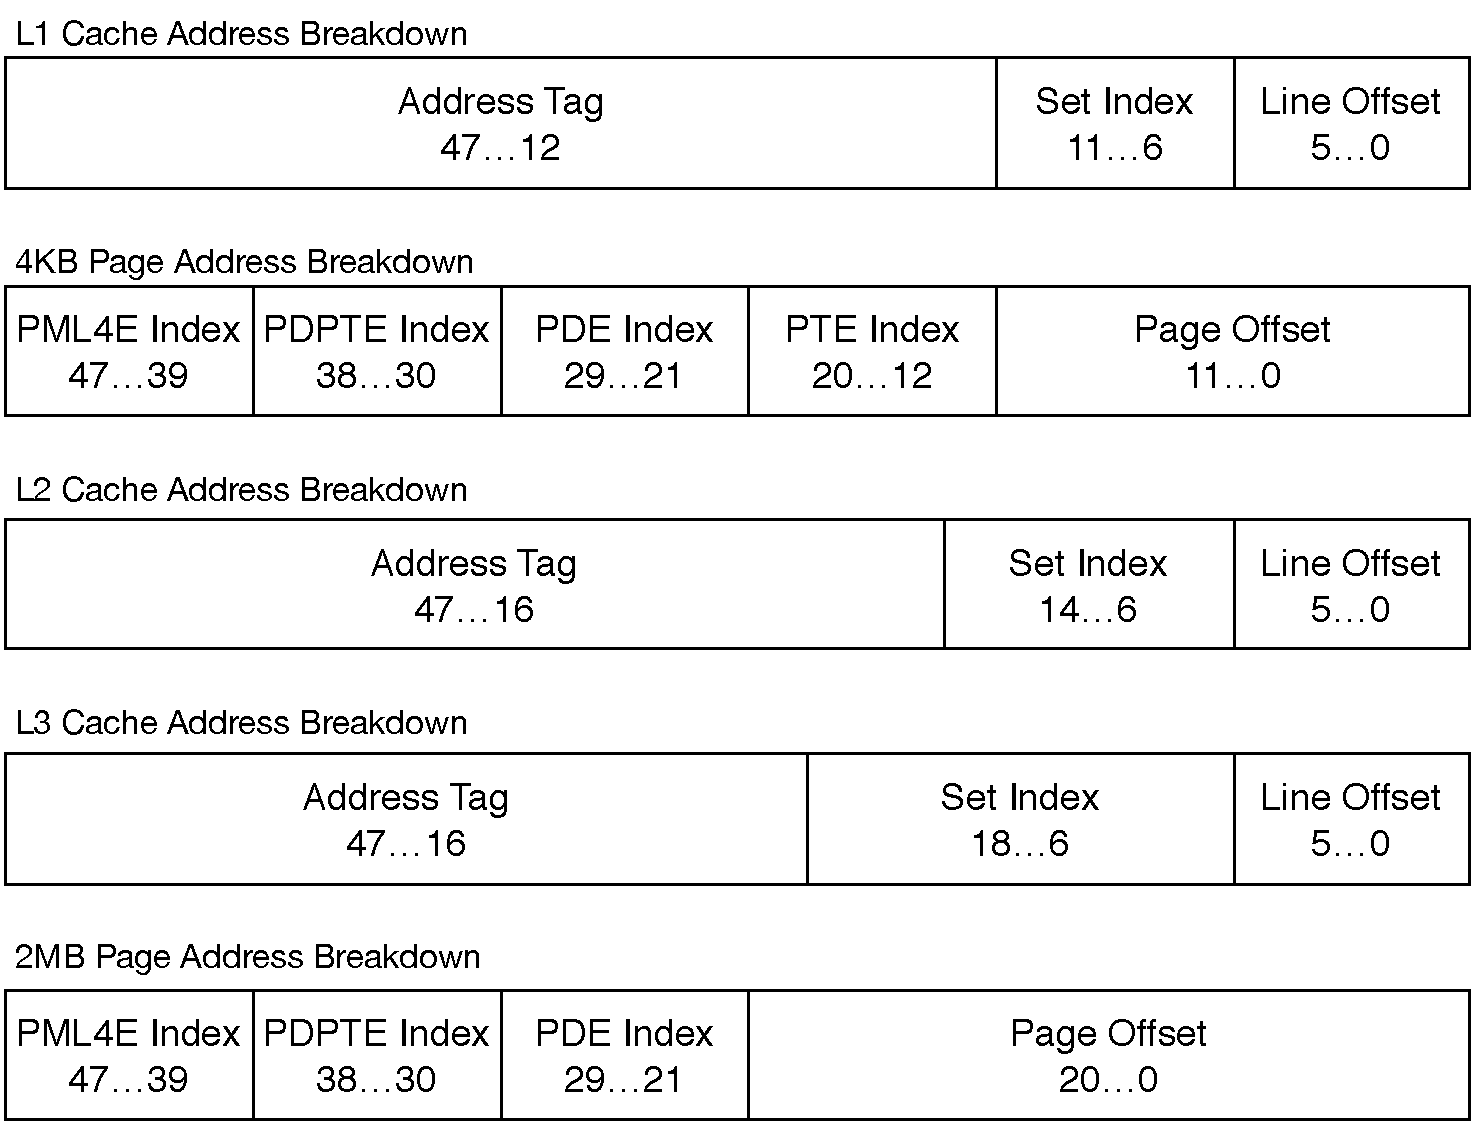
\includegraphics[width=85mm]{figures/caching_and_paging.pdf}}
  \caption{
    Virtual addresses from the perspective of cache lookup and address
    translation. The bits used for the L1 set index and line offset are not
    changed by address translation, so the page tables do not impact L1 cache
    placement. Page tables do impact L2 and L3 cache placement. Using large
    pages (2MB or 1GB) makes cache placement independent of page tables.
  }
  \label{fig:caching_and_paging}
\end{figure}

The L2 cache in recent Intel processors uses physical indexing
\cite{patterson2013architecture}. The indexing method is not documented in
Intel's manuals and is not reported by the CPUID instruction, as it is
considered to be an implementation detail. However, the indexing method
determines the set index for a given memory location, and knowing which memory
addresses are stored in the same set is crucial for mounting and defending
against cache timing attacks.

\begin{figure}[hbt]
  \center{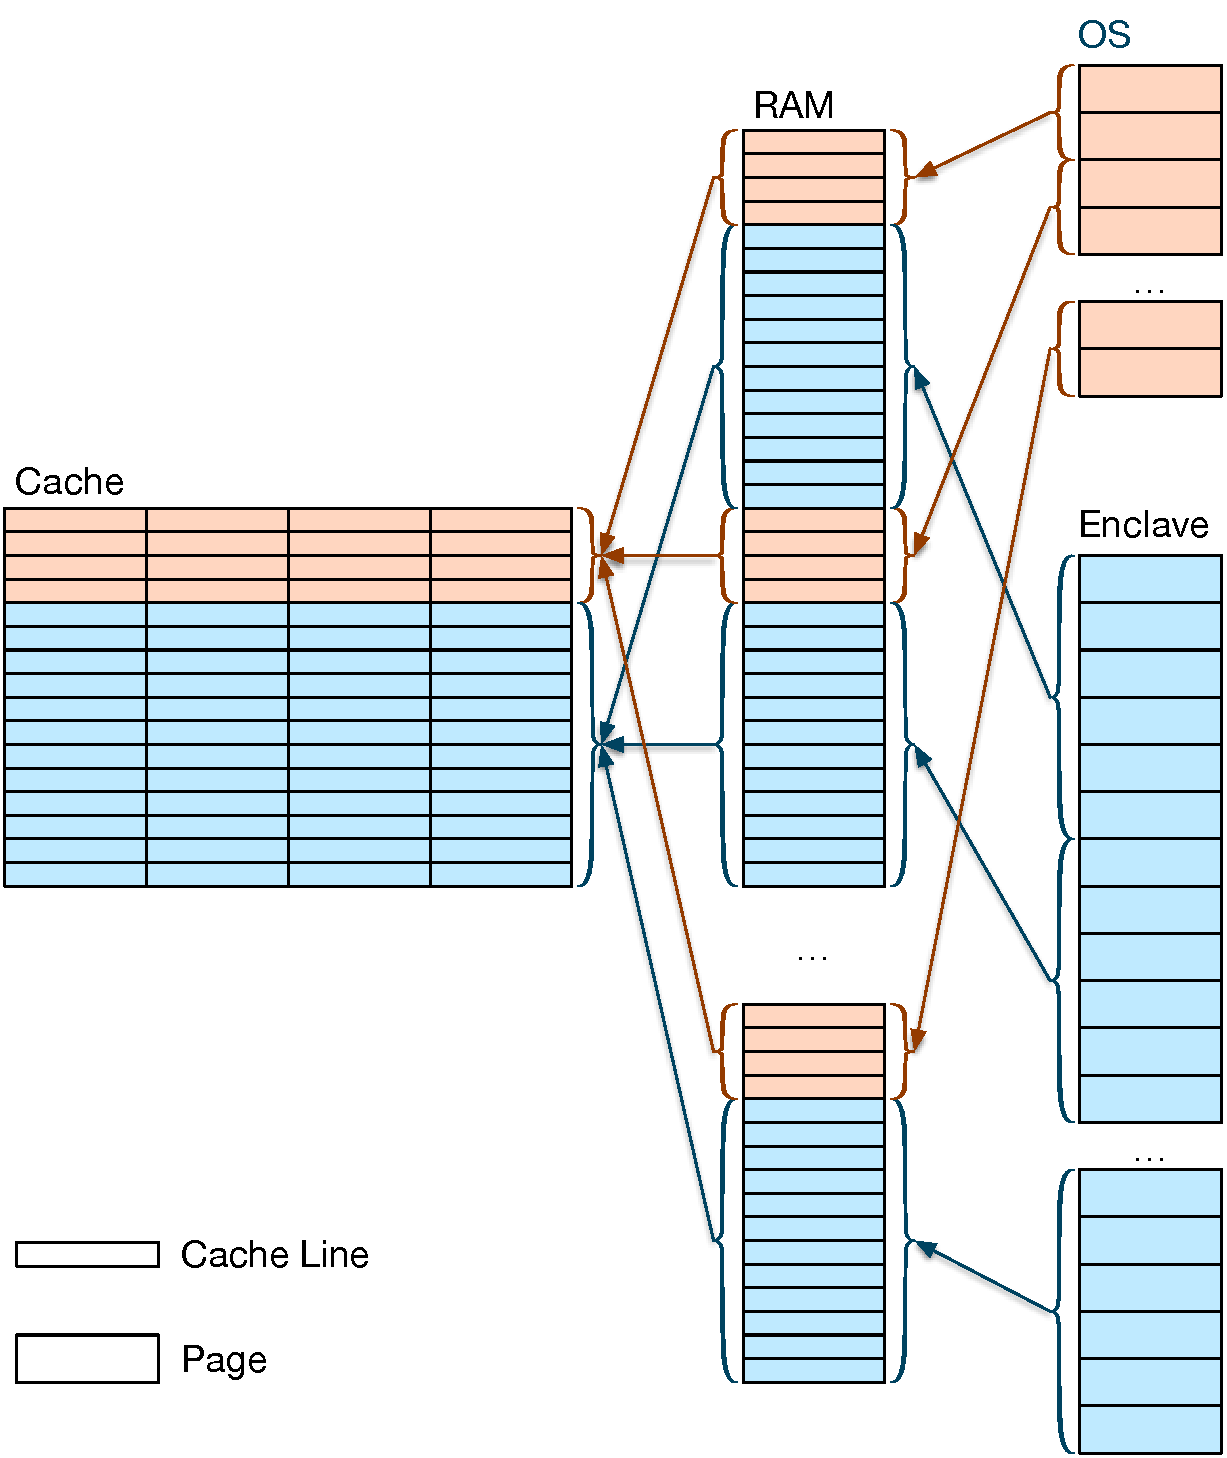
\includegraphics[width=85mm]{figures/cache_partitions.pdf}}
  \caption{
    Cache partitioning between two applications. Each application has some
    cache sets allocated to it, and only uses RAM regions that map to its cache
    sets. When partitioning the L1 cache, applications have to follow this
    constraint themselves. When the L2 cache is partitioned, the OS can map the
    pages in an application's virtual address space to the RAM regions that the
    application can use, so applications are oblivious to the cache
    partitioning.
  }
  \label{fig:cache_partitions}
\end{figure}
